\documentclass{article}
\usepackage[utf8]{inputenc}
\usepackage{lipsum}
\usepackage[left=2cm, right=2cm, top=3cm, includefoot]{geometry}
\usepackage{comment}
\usepackage {graphicx}%Import images
\usepackage{float}%Set any float position of images for example.
\usepackage{titlepic}


\graphicspath{ {\Users\soren\Desktop\Projects 5. semester\Big Data/} }


%Allows for different colors in report
\usepackage{color}
\usepackage[dvipsnames, table, xcdraw]{xcolor}

%Setup allows for clickable ToC with different colors
\usepackage{hyperref}
\hypersetup{
    colorlinks,
    citecolor=black,
    filecolor=black,
    linkcolor=black,
    urlcolor=black
}


% Header and Footer Stuff
\usepackage{fancyhdr}
\pagestyle{fancy} %Use fancy page style
\fancyhead[R]{CBS} %Align to the right on the page
\fancyfoot{}
\fancyfoot[R]{\thepage\ } %Align to the right on the page
\renewcommand{\headrulewidth}{0.5pt} %overwrite headers width
\renewcommand{\footrulewidth}{1pt}  %overwrite footers width




\begin{comment}
Renew command overwrites a previous function. Therefore, it is used to overwrite the header and footer width.
fancyfootHDR package, allows us to add cool headers and footers. R aligns to the right  \thepage\ references the actual page number.
\end{comment}




%
\begin{document}





%Start of titlepage
\begin{titlepage}
	\begin{center}
	\line(1,0){300} \\
	[0.25in]
	\color{NavyBlue} \huge{\bfseries A Big Data Research Paper} \\   
	[2mm]	
	\color{black}
	\line(1,0) {200} \\
	[0.1cm]
	\color{black}\textsc{\LARGE On Donald J. Trump's Twitter Activity} \\
	[0.75cm]
	\textsc{\LARGE Copenhagen Business School} \\
	[9.5cm]




\end{center}



\begin{figure}[H]
	\centering

%
 %\raisebox{20mm}[0pt][0pt]{
 %\makebox[\textwidth][c]{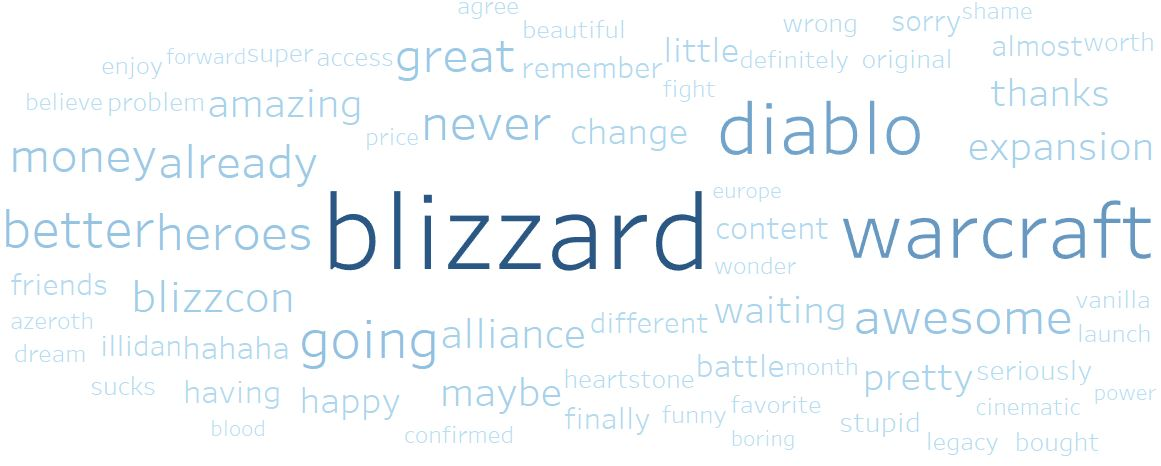
\includegraphics[scale=.55]{BlizzardWord2Cloud.PNG}
 %}}

\vspace*{-12cm} 
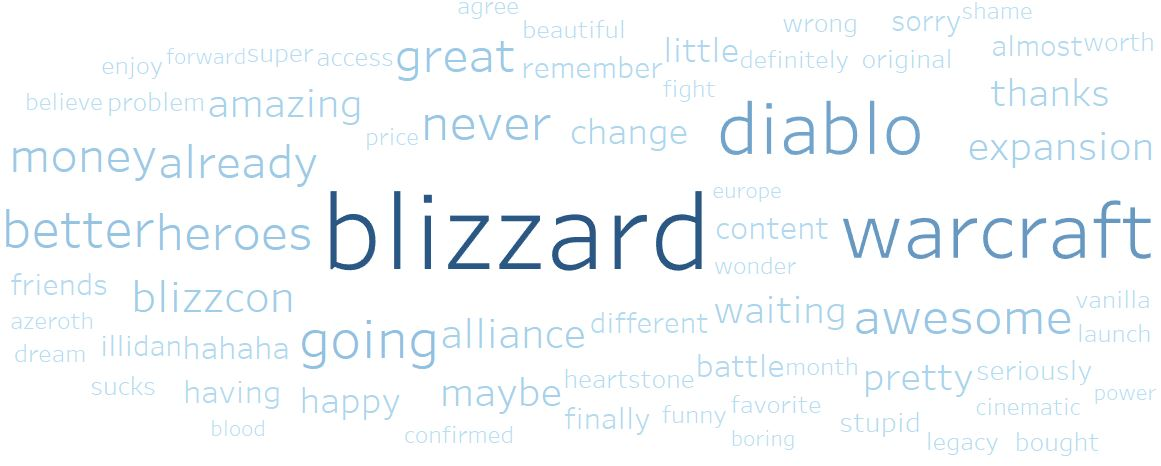
\includegraphics[scale=.55]{BlizzardWord2Cloud.PNG}



\caption{ Blizzard Wordcloud }
\vspace*{1.25cm} 


\end{figure}


	\begin{flushright}
\vspace*{1.25cm} 

	\textsc{\large Søren Kolbye Jensen \\}
	Bsc. Ha(IT) \\
	\#43124133123 \\
	December 1, 2017
	\end{flushright}





%End of titlepage
\end {titlepage}



%Table of contents & summary
\color{NavyBlue} \tableofcontents \color{black}
\thispagestyle{empty} %Remove the header, by removing all the style
 \cleardoublepage
\setcounter{page}{1}%Reset page counter at introduction page 
\pagenumbering{arabic}
%\addcontentsline{toc}{section}{\numberline{}Summary}


\cleardoublepage%Table of contents end


\section{Summary} %Summary
Summary section


\cleardoublepage %Summary end


%End of table of contents & summary









%Start of report






%Start of introduction_____________________________________________


\color{NavyBlue} \section{Introduction} \label{sec:intro}

\color {black}

Big Data has changed how data is viewed in society, businesses have  invested heavily in infrastructure that can imrpove data collection.
It is now possible, to use Big Data to analyze the behaviour of Social Media channels such as Twitter, Facebook and Instagram.


These principles are called "Datascience and Datamining". According to (INSERT BOOK), datascience and datamining can be defined as follows:

Data science is the act of using fundamental principles, to guide extraction of knowledge from datasets.

Datamining on the other hand, deals with extracting knowledge from data using technolgoies, which incorporates the principles of data science. 

This research paper, aims to use the fundamental principles of Data science, in conjunction with  datamining technologies. 
To analyze the behvaiour of U.S president Donald J. Trump. and how this behaviour affected his political campaign, as well as how his behaviour affected the American financial markets.



%Big Data  book ch1


\begin{figure}[H] %We begin our figure and want it to stay H(ere)
	\centering %We want to center the figure
\fbox{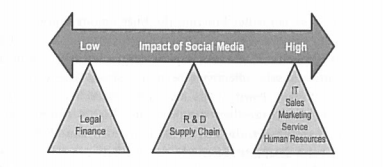
\includegraphics [scale= 1.25]  {Threefactor.PNG}    } %Include our ijmage with a height and location of img.
	\caption[Optional caption] {real, local caption for refrence}
	\label{fig:wordcloudBliz}

\end{figure}






\subsection{Case introduction}
Donald John Trump, born in 1946 in Queens New York, is the CEO of the Trump Organization and is well known as a real-estate broker in the United States.
However, on june 16th, 2015, Trump officially announced his candidacy as the 20th US President". This political campaign was heavily involved with Social Media, as Trump was actively fighting big news channels, such
as CNN, NBC etc. labelling them as "fake news". Thus, Trump figured out a way to distribute highly controversial statements and gain political support by his use of Social Media Channels such as Twitter. 


%http://secfilings.nasdaq.com/edgar_conv_html%2f2017%2f02%2f28%2f0001047469-17-001072.html#FIS_BUSINESS

\cleardoublepage



%End of introduction________________________________

%https://www.aol.com/2016-election/timeline/
%https://www.dropbox.com/sh/kd87npmrvcwiyge/AADRTmSB6lDt5ChunVY_Xy0Ea/ExampleProjects?dl=0&preview=ExampleProject%2301-VisualAnalytics-NYC_TaxiRides-GreenCabs_vs_Uber.pdf

\section{Problem Formulation and Reserach questions} \label{sec:ch1}
The goal of this research paper is to analyze  trumps behaviour on Twitter and how he used Twitter to combat "fake news". A visual analysis on his behaviour between DATE and DATE will be conducted to reveal the patterns in his behaviour in this timeframe. This leads to the reserach question: 

\par\vspace{10pt}

What was trump's behaviour on social media, prior to his announcement of his presidency. And how did it change, during and after his political campaign.

\par\vspace{10pt}

Furthermore, Trump's political campaign was heavily focused on combating illegal immigration. One of the primary targets of Trump's statement was Mexico.
This leads to the research question:

How did Trump's political statements on Twitter affect the American and Meixcan currency.

\par\vspace{10pt}






\subsection{Something}



%Methodology start

\section{Methodology}
Insert introduction to the methodology section of the report


\begin{table}[H]
\centering
\caption{My caption}
\label{my-label}
\begin{tabular}{|
>{\columncolor[HTML]{FFFFFF}}l |
>{\columncolor[HTML]{FFFFFF}}l |
>{\columncolor[HTML]{FFFFFF}}l |
>{\columncolor[HTML]{FFFFFF}}l |
>{\columncolor[HTML]{FFFFFF}}l |}
\hline
{\color[HTML]{000000} \textbf{Hej}} & {\color[HTML]{000000} dsa} & {\color[HTML]{000000} dasdsad} & {\color[HTML]{000000} asdasd} & {\color[HTML]{000000} asdsa} \\ \hline
{\color[HTML]{000000} \textbf{asd}} & {\color[HTML]{000000} dsfdsfs} & {\color[HTML]{000000} adsad} & {\color[HTML]{000000} asdasd} & {\color[HTML]{000000} asd} \\ \hline
{\color[HTML]{000000} \textbf{asdad}} & {\color[HTML]{000000} xcvx} & {\color[HTML]{000000} sadada} & {\color[HTML]{000000} asdaa} & {\color[HTML]{000000} sa} \\ \hline
{\color[HTML]{000000} \textbf{adsada}} & {\color[HTML]{000000} sad} & {\color[HTML]{000000} dasd} & {\color[HTML]{000000} ada} & {\color[HTML]{000000} dasd} \\ \hline
\end{tabular}
\end{table}




\subsection{Data Acquisition and Dataset Description}
The datasets in this research paper has been collected from Trump's Twitter page, ranging from 2009 to 2017.

The first datasets consists of Twitter data on Trump's primary twitter channel. 

The second dataset consists of Historical data on the American and Mexican currency between Trump's announcement to  14/07/2017

05/04/2009
07/14/2017


%End of report__________________________________



\end{document}






%\begin{figure}[H] %We begin our figure and want it to stay H(ere)
%	\centering %We want to center the figure


 %\raisebox{10mm}[0pt][0pt]{
%\fbox{ \makebox[\textwidth][c]{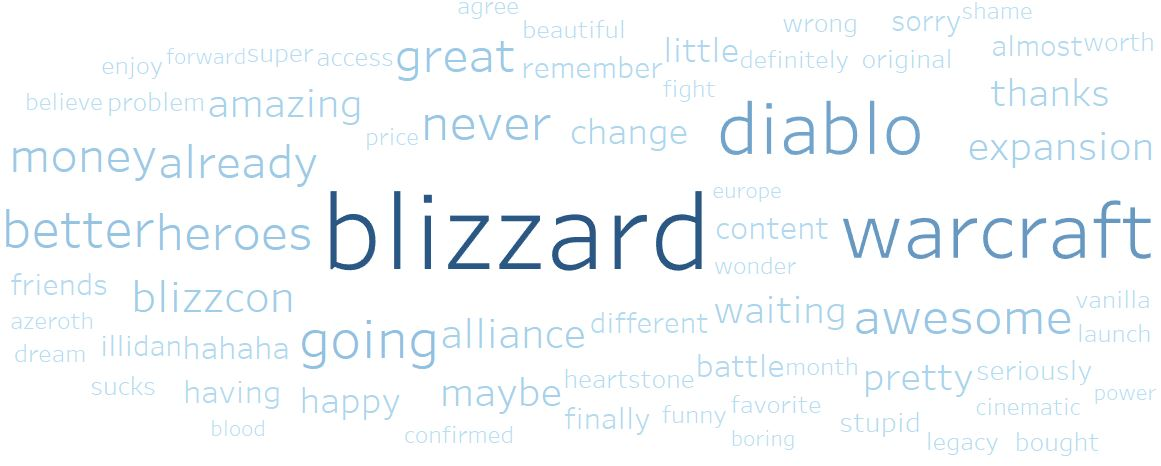
\includegraphics[scale=.55]{BlizzardWord2Cloud.PNG}}
% }}
%\vspace*{-40mm} %Close in the caption to the image

%\protect\caption[position=bottom]{Title of Figure\label{fig:F1}}


%\vspace{3cm}
%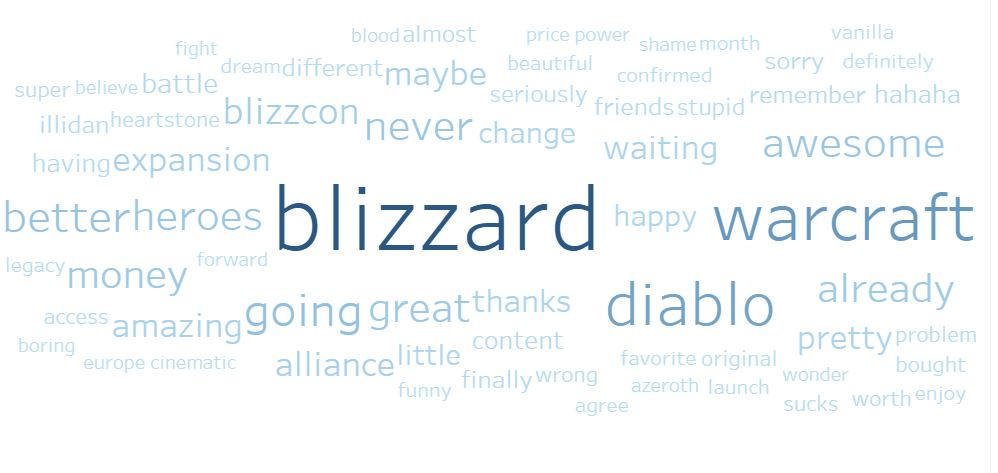
\includegraphics [width = 7in]  {BlizzardWordCloud.PNG}     %Include our ijmage with a height and location of img.
	
%	\label{fig:wordcloudBliz}

%\end{figure}



